% libroResMat2
% Copyright (C) 2020  J.M. Perez Zerpa, et. al.
%
% This program is free software: you can redistribute it and/or modify
% it under the terms of the GNU General Public License as published by
% the Free Software Foundation version 3 of the License.
%
% This program is distributed in the hope that it will be useful,
% but WITHOUT ANY WARRANTY; without even the implied warranty of
% MERCHANTABILITY or FITNESS FOR A PARTICULAR PURPOSE. See the
% GNU General Public License for more details.
%
% You should have received a copy of the GNU General Public License
% along with this program.  If not, see <http://www.gnu.org/licenses/>.

\chapter{Estructuras tridimensionales de barras}

\section{Emparrillados}

En esta sección se presentan de forma esquemática los conceptos más importantes para la determinación de desplazamientos y solicitaciones en estructuras planas de barras, sometidas a fuerzas perpendiculares al plano de la estructura. %
%
Estas estructuras, tal como fue visto en la Sección~\ref{sec:clasifest}, son llamadas estructuras planoespaciales o emparrillados.

\subsection{Torsión}


En cursos anteriores se abordó la teoría de torsión de Saint-Venant para vigas de sección transversal con doble eje de simetría. %
%
A continuación se enumeran algunas de las magnitudes y conceptos más importantes, utilizando el enfoque utilizado en \citep{Wunderlich2002}.

Sea una barra con un extremo empotrado sometida a un momento torsor $M_t$ se verifica:
%
\begin{equation}
M_t = G J \Theta
\end{equation}
donde $G$ es el módulo de corte, dado por
\begin{equation}
G=\frac{E}{2(1+\nu)},
\end{equation}
$\Theta$ es el barrenado dado por el cociente entre el ángulo de giro del extremo libre y el largo  $\Theta = \theta / \ell$, y $J$ es la inercia torsional de la sección dada por:
%
\begin{equation}
J = \int_{A} \psi_P \dif A.
\end{equation}
%
En esta última expresión $\psi_P$ representa la función de Prandtl, dada por la solución del siguiente problema en derivadas parciales:
%
\begin{equation}
\left\{
\begin{array}{lr}
\Delta \psi_P = -2 & \text{en} \, A\\
\psi_P = 0 & \text{en} \, \partial A
\end{array}
\right.
\end{equation} 
%

Si se considera un elemento con giros nodales $\theta_1$ y $\theta_2$ se tiene:
%
\begin{equation}
  M_t = G J \frac{\theta_2 - \theta_1}{\ell}
\end{equation}

Por otra parte la energía de deformación torsional está dada por:
%
\begin{equation}
\Pi_{int,\text{torsión}}(\theta_1,\theta_2) = \frac{1}{2} \frac{G J}{\ell} \left( \theta_2 - \theta_1\right)^2.
\end{equation}
%

A partir de la relación entre $\psi_P$ y las tensiones rasantes se puede calcular también el valor de la tensión rasante máxima debida a torsión, dado por:
%
\begin{equation}
\tau_{max} = \frac{M_t}{W_t}
\end{equation}
%
donde $W_t$ es el módulo resistente torsional.


\subsection{Barras sometidas a flexo-torsión}
%
En esta sección se presentan las ecuaciones que relacionan los desplazamientos y fuerzas para barras sometidas a flexión y torsión. %
%
Esto puede ser considerado como una extensión de lo que se vió en la Sección~\ref{sec:mdvig}. %

Se considera un elemento de barra de largo $\ell$ con inercia flexional $I_z$ e inercia torsional $J$. %
%
Las fuerzas nodales consideradas son: por una parte fuerzas y flectores tales que la flexión se produce en el plano formado por los vectores $\bfe_x$ y $\bfe_y$, y por otra parte momentos torsores tales que el vector director (regla de mano derecha) está orientado según el eje $\bfe_x$. %


En general se considera que existe un sistema de coordenadas global  $x,y,z$ y el eje del elemento forma un ángulo $\alpha_y$ con el eje $\bfe_x$ global tal como se muestra en la \autoref{fig:vigators}. %
El ángulo $\alpha_y$ es medido positivo desde el eje $\bfe_x$ global al local con la regla de la mano derecha según el eje $-\bfe_y$.


\begin{figure}[htb]
	\centering
  \def\svgwidth{1\textwidth}
  \input{figs/UT5/viga3d_torsion.pdf_tex}
  \caption{Esquema de elemento de barra a flexo-torsión. Sistemas de coordenadas locales (L) y coordenadas globales representados.}
  \label{fig:vigators}
\end{figure}


En la figura se encuentran representados tanto momentos como giros nodales, donde se considera que los giros y momentos se representan con la misma convención de signo. %
%

Considerando que la barra pertenece al plano $x,z$ se puede descomponer los vectores de momentos y giros en coordenadas locales en una base de coordenadas globales, de la forma:
%
\begin{eqnarray}
M_{x,1,L} &=& \cos(\alpha_y) M_{x,1} + \sin(\alpha_y) M_{z,1} \\
M_{z,1,L} &=& - \sin(\alpha_y) M_{z,1} + \cos(\alpha_y) M_{x,1}
\end{eqnarray}

Considerando también la fuerza según $y$ se tiene:
\begin{eqnarray}
M_{x,1,L} &=& \cos(\alpha_y) M_{x,1} + \sin(\alpha_y) M_{z,1} \\
F_{y,1,L} &=& F_{y,1} \\
M_{z,1,L} &=& - \sin(\alpha_y) M_{z,1} + \cos(\alpha_y) M_{x,1}
\end{eqnarray}

De forma equivalente para los desplazamientos y giros se tiene:
\begin{eqnarray}
\theta_{x,1,L} &=& \cos(\alpha_y) \theta_{x,1} + \sin(\alpha_y) \theta_{z,1} \\
v_{y,1,L} &=& v_{y,1} \\
\theta_{z,1,L} &=& - \sin(\alpha_y) \theta_{z,1} + \cos(\alpha_y) \theta_{x,1}
\end{eqnarray}
%
y expresiones equivalentes para el nodo 2.

Definiendo el vector de desplazamientos nodales en coordenadas globales:
\begin{equation}
\bfu = 
\left[
\begin{matrix}
\theta_{x,1} & v_{y,1} & \theta_{z,1} & \theta_{x,2} & v_{y,2} & \theta_{z,2}
\end{matrix}
\right]^T
\end{equation}
%
y el vector de desplazamientos nodales en coordenadas locales:
\begin{equation}
\bfu_L = 
\left[
\begin{matrix}
\theta_{x,1,L} & v_{y,1,L} & \theta_{z,1,L} & \theta_{x,2,L} & v_{y,2,L} & \theta_{z,2,L}
\end{matrix}
\right]^T
\end{equation}
%
se puede representar la relación entre desplazamientos en diferentes sistemas de coordenadas como:
%
\begin{equation}\label{eqn:matrot}
\bfu = \bfR \bfu_L
\end{equation}
donde
\begin{equation}
\bfR = 
\left[
\begin{matrix}
\cos(\alpha_y) & 0  & -\sin(\alpha_y) & 0 & 0 & 0\\
 0 & 1 & 0 &  0 & 0 & 0\\
\sin(\alpha_y) & 0  & \cos(\alpha_y) & 0 & 0 & 0\\
%
0 & 0 & 0 & \cos(\alpha_y) & 0  & -\sin(\alpha_y) \\
0 & 0 & 0 & 0 & 1 & 0 \\
0 & 0 & 0 & \sin(\alpha_y) & 0  & \cos(\alpha_y)
\end{matrix}
\right].
%
\end{equation}


Esta matriz de rotación puede ser obtenida también aplicando los conceptos de algebra lineal de matriz de cambio de base.

La energía potencial de deformación total está dada por la suma de las energías potenciales debidas a torsión y flexión, las cuales pueden ser representadas en coordenadas locales como:
%
\begin{equation}
\Pi_{int} (\bfu_L ) = \Pi_{int,\text{torsión}}(\theta_{x,1,L},\theta_{x,2,L}) + \Pi_{int,\text{flexión}}(v_{y,1,L}, \theta_{z,1,L},v_{y,2,L},\theta_{z,2,L})
\end{equation}
%
donde $\Pi_{int,\text{flexión}}$ está dada por la Ecuación~\eqref{eqn:Uflex}. %
%
La energía potencial de las fuerzas externas está dada por $\Pi_{ext} (\bfu_L) = -\bfu_L^T \bff_L$ donde $\bff_L$ está dado por:
\begin{equation}
\bff_L = 
\left[
\begin{matrix}
	M_{x,1,L} & F_{y,1,L} & M_{z,1,L} & M_{x,2,L} & F_{y,2,L} & M_{z,2,L}
\end{matrix}
\right]^T.
\end{equation}


Utilizando el principio de mínima energía potencial total y aplicando las condiciones del primer teorema de Castigliano se tienen las siguientes cuatro condiciones para flexión:
\begin{eqnarray}
\frac{\partial \Pi_{int,\text{flexión}}}{\partial v_{y,1,L}} =  F_{y,1,L}  \qquad \frac{\partial \Pi_{int,\text{flexión}}}{\partial \theta_{z,1,L}} =  M_{z,1,L} \\
\frac{\partial \Pi_{int,\text{flexión}}}{\partial v_{y,2,L}} =  F_{y,2,L} \qquad \frac{\partial \Pi_{int,\text{flexión}}}{\partial \theta_{z,2,L}} =  M_{z,2,L}
\end{eqnarray}
y las siguientes condiciones para torsión:
%
\begin{equation}
\frac{\partial \Pi_{int,\text{torsión}}}{\partial \theta_{x,1,L}} =  M_{x,1,L} \qquad 
\frac{\partial \Pi_{int,\text{torsión}}}{\partial \theta_{x,2,L}} =  M_{x,2,L}
\end{equation}

Sustituyendo las expresiones de las energías de deformación se obtiene que las condiciones de Castigliano son equivalentes al sistema de ecuaciones:
\begin{equation}
\bfK_L \bfu_L = \bff_L
\end{equation}
%
donde la matriz $\bfK_L$ es la matriz de rigidez en coordenadas locales, dada por:
%
\begin{equation}\label{eqn:matrigtf}
	\bfK_L = \left[
	\begin{matrix}
		\dfrac{GJ}{\ell} & 0 & 0 & - \dfrac{GJ}{\ell} & 0 & 0 \\[3mm]
		%
		0 &  12 \dfrac{EI_z}{\ell^{3}} & 6 \dfrac{EI_z}{\ell^{2}} &  0& -12 \dfrac{EI_z}{\ell^{3}} & 6 \dfrac{EI_z}{\ell^{2}} \\[3mm]
		0 &  6 \dfrac{EI_z}{\ell^{2}} & 4 \dfrac{EI_z}{\ell} & 0& -6 \dfrac{EI_z}{\ell^{2}} & 2 \dfrac{EI_z}{\ell} \\[3mm]
		-\dfrac{GJ}{\ell} & 0 & 0 &  \dfrac{GJ}{\ell} & 0 & 0 \\[3mm]
		%
		0 &  -12 \dfrac{EI_z}{\ell^{3}} & -6 \dfrac{EI_z}{\ell^{2}} &0&  12 \dfrac{EI_z}{\ell^{3}} & -6 \dfrac{EI_z}{\ell^{2}} \\[3mm]
		0 &  6 \dfrac{EI_z}{\ell^{2}} & 2 \dfrac{EI_z}{\ell} & 0 & -6 \dfrac{EI_z}{\ell^{2}} & 4 \dfrac{EI_z}{\ell} \\[3mm]
	\end{matrix}
	\right].
\end{equation}

Utilizando que $\bfu_L = \bfR^T \bfu$  y que  $\bff_L = \bfR^T \bff$  se obtiene el sistema en coordenadas globales:

\begin{equation}
\bfK \bfu = \bff
\end{equation}

donde la matriz de rigidez $\bfK$ es la matriz de rigidez en coordenadas globales dada por
\begin{equation}\label{eqn:matrigtfglo}
\bfK = \bfR \bfK_L \bfR^T.
\end{equation}

Para un emparrillado formado por $n$ elementos de barra se debe calcular cada matriz en coordenadas globales y realizar el ensamblado de forma similar a como es realizado para elementos de reticulados o pórticos. %
%

\subsection{Ejemplo}

Sea la estructura mostrada en la Figura~\ref{fig:UT5_ejemplo}, donde todas las barras tienen inercia flexional $I$ e inercia torsional $J$ a determinar y están formadas por un material de módulo de Young $E$. %
Se considera que $E=210$ GPa, $\nu=0.3$, $\ell=2 $ m, la sección transversal es cuadrada de lado $5$ cm. %
%
Se desea calcular los desplazamientos nodales para una carga puntual $P=4 $ kN.

\begin{figure}[htb]
	\centering
	\def\svgwidth{0.6\textwidth}
	\input{figs/UT5/UT5_ejemplo.pdf_tex}
	\caption{Esquema básico de cálculo de ejemplo de emparrillado.}
	\label{fig:UT5_ejemplo}
\end{figure}

La barra con la carga puntual aplicada tiene una geometría y condiciones de vínculo simétricos por lo que el giro $\theta_x$ debe ser nulo.
%
Considerando está condición de simetría  y dividiendo la estructura en dos mitades, se obtiene el esquema básico simplificado que se muestra en la Figura~\ref{fig:UT5_ejemplo2}.

\begin{figure}[htb]
	\centering
	\def\svgwidth{0.7\textwidth}
	\input{figs/UT5/UT5_ejemplo_connodos.pdf_tex}
	\caption{Esquema de mitad de estructura de ejemplo de emparrillado.}
	\label{fig:UT5_ejemplo2}
\end{figure}

Utilizando la numeración definida, se establece la conectividad de los elementos como Elemento 1: del nodo 1 al 2 y Elemento 2: del nodos 2 al 3. %
Los sistemas de coordenadas locales considerados se muestran en la figura.

Para el cálculo de las matrices de rigidez cada elemento se usa la expresión de la Ecuación~\eqref{eqn:matrigtfglo}.

Para el elemento 1, $\bfK_L$ está dada por la expresión de la ecuación~\eqref{eqn:matrigtf} y $\bfR$ es la matriz identidad de tamaño $6\times6$.

Para el elemento 2, $\bfK_L$ es calculada considerando el largo $\ell/2$ en la ecuación~\eqref{eqn:matrigtf} y para la matriz de rotación se considera $\alpha_y=-\pi/2$ en la ecuación \eqref{eqn:matrot} por lo tanto
\begin{equation}
\bfR = 
\left[
\begin{matrix}
0 & 0  & 1 & 0 & 0 & 0\\
0 & 1 & 0 &  0 & 0 & 0\\
-1 & 0  & 0 & 0 & 0 & 0\\
%
0 & 0 & 0 & 0 & 0  & 1 \\
0 & 0 & 0 & 0 & 1 & 0 \\
0 & 0 & 0 & -1 & 0  & 0
\end{matrix}
\right].
%
\end{equation}


El módulo de corte es $G=80.7 $ GPa. La inercia flexional es $I= 5.208 \times 10^{-7}$ m$^4$, la inercia flexional $J= 0.141 (0.05)^4 = 8.81 \times 10^{-7}$ m$^4$.

Los desplazamientos para el nodo 2 son:

$$
\theta_{x,2} = -0.022154
\quad 
v_2 = -0.048762 
\quad
\theta_{z,2} = -0.036571
$$

Y para el nodo 3 son
$$
v_3 = -0.083107
\quad
\theta_{z,3} = 
-0.036571
$$


\subsection{Implementación computacional}

En el Código~\ref{cod:emparrillados} en la Sección~\ref{sec:codut5} se presenta una implementación en GNU-Octave del método descrito y su aplicación para la resolución del ejemplo visto. %
%
El código ha recibido aportes y modificaciones de estudiantes del curso 2019, los nombres de los autores de los aportes fueron agregados al código y los cambios están visibles en el repositorio\footnote{\href{https://gitlab.fing.edu.uy/jorgepz/emparrillados/commits/master}{https://gitlab.fing.edu.uy/jorgepz/emparrillados/commits/master}.}


\section{Estructuras tridimensionales de barras}

En el caso de estructuras tridimensionales, los elementos de barra pueden estar sometidos a esfuerzos de fuerzas y momentos que producen 6 solicitaciones internas: directa, torsión, 2 flectores y 2 cortantes (correspondientes a la flexión en los dos planos definidos por los ejes de coordenadas locales transversales).

\subsection{Elemento de viga sometido a flexo compresión esviada}

El caso de flexión esviada corresponde a vigas sometidas a momentos flectores con componentes no nulas en los dos ejes de coordenadas locales transversales (siendo estos los ejes de los momentos de inercial principales). %

El desarrollo de las ecuaciones para vigas sometidas a esfuerzos axiales y transversales es equivalente al presentado en la Sección~\ref{sec:teoviga}, considerando que los giros de las secciones son no nulos tanto en el eje $y$ como el eje $z$, esto es $\theta_z \neq 0$ y $\theta_y \neq 0$. %
%
Al mismo tiempo se tiene que ambos desplazamientos transversales $v$ y $w$ son no nulos.

También se mantiene la hipótesis de que caras planas permanecen planas, por lo que el desplazamiento de un punto ubicado en un punto con coordenadas $x,y,z$ puede ser escrito como:
%
\begin{equation} \label{eqn:despaxidosdir}
  u(x,y,z) = u_G(x) - y \theta_z(x) + z \theta_y(x).
\end{equation}

Realizando un desarrollo equivalente al del caso plano se puede obtener las relaciones 
%
\begin{equation}
 \theta_z(x) = \frac{\partial v}{\partial x}(x), \qquad  \theta_y(x) = - \frac{\partial w}{\partial x}(x),
\end{equation}
%
y la expresión de la tensión axial:
%
\begin{equation}\label{eqn:tensaxiflexesv}
\boxed{
	\sigma(x,y,z) = \frac{	N (x) }{A}
	- y \frac{	M_z (x) }{I_z} + z \frac{	M_y (x) }{I_y} 
}
\end{equation}

En clase se presentará el razonamiento utilizado en este desarrollo así como también se verán ejemplos prácticos.




\subsection{Elemento de pórtico tridimensional}

En clase se presentará brevemente el elemento de barra tridimensional, el cual es considerado sometido a torsión, flexión en ambos planos (es decir \textit{flexión esviada}) y directa. %
%
Este es el elemento de viga que se encuentra implementado en el código ONSAS, utilizado en clases de teórico para resolver problemas de pórtico 3D.


\section{Ejercicios}
\setcounter{ejercicio}{0}

\ejercicio

Sea la estructura mostrada en la figura, construida con caños de acero ($E=210$ GPa y $\nu =0.3$) de $\phi_{ext} = 100$ mm y $t=8$ mm.

\begin{center}
	\def\svgwidth{0.5\textwidth}
	\input{./figs/UT5/UT5_ej1.pdf_tex}
\end{center}

Considerando $P=4$ kN y $L=1.0$ m, se pide:
%
\parte Calcular los desplazamientos y giros nodales y trazar diagramas de solicitaciones usando:
\begin{enumerate}
\item Equilibrios y valores de deflexiones y giros en ménsulas. 
\item Análisis matricial.
\end{enumerate}
\parte Comparar los resultados hallados en a) con los obtenidos mediante:
  \begin{enumerate}
   \item una versión modificada del código \ref{cod:emparrillados}
  \item alguna de las herramientas computacionales presentadas en el curso
  \end{enumerate}


\ejercicio

Se construye un emparrillado con caños de acero (E=210 GPa, $\nu=0.3$) de $\phi_{ext}=100$ mm y $t=8$ mm, sometido a dos estados de carga mostrados en las figuras.

\begin{center}
	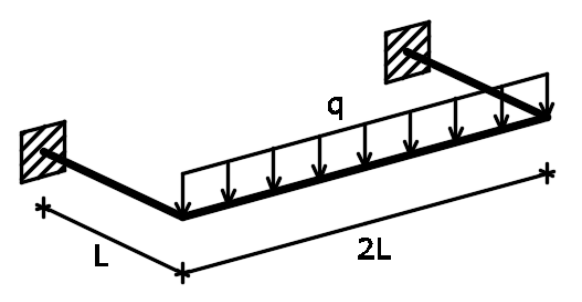
\includegraphics[width=0.4\linewidth]{UT5ej2a}
	\hspace{0.1\linewidth}
	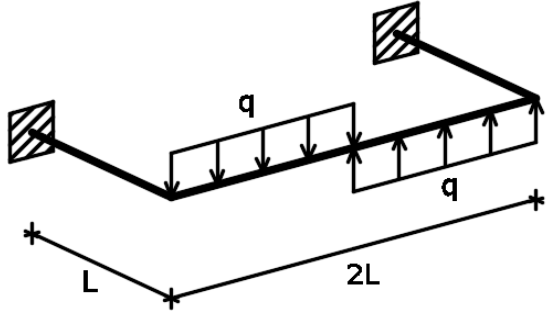
\includegraphics[width=0.4\linewidth]{UT5ej2b}
\end{center}

Considerando $q=2$ kN/m y $L=1$ m, se pide:

\parte Resolver mediante el método de análisis matricial, considerando la simetría o antisimetría del problema para trabajar con una cantidad de barras reducida.
\parte Trazar diagramas de solicitaciones y comparar con los obtenidos con un modelo computacional de la estructura.

\vspace{1cm}
El emparrillado analizado es ahora usado como parte de la estructura de una hamaca con su respectivo esquema básico de cálculo como se muestra en las figuras. %
Las cargas $q$ consideradas en las partes anteriores se aplican únicamente en la barra EF.

\begin{center}
	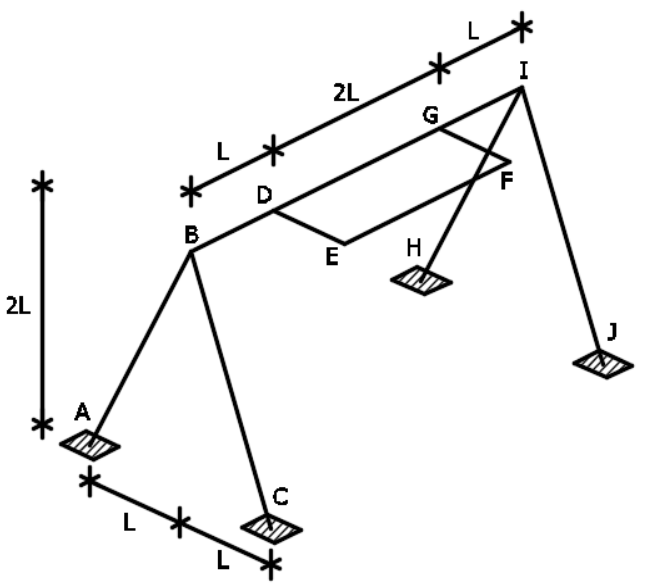
\includegraphics[width=0.5\linewidth]{UT5ej2c}
	\hspace{0.05\linewidth}
	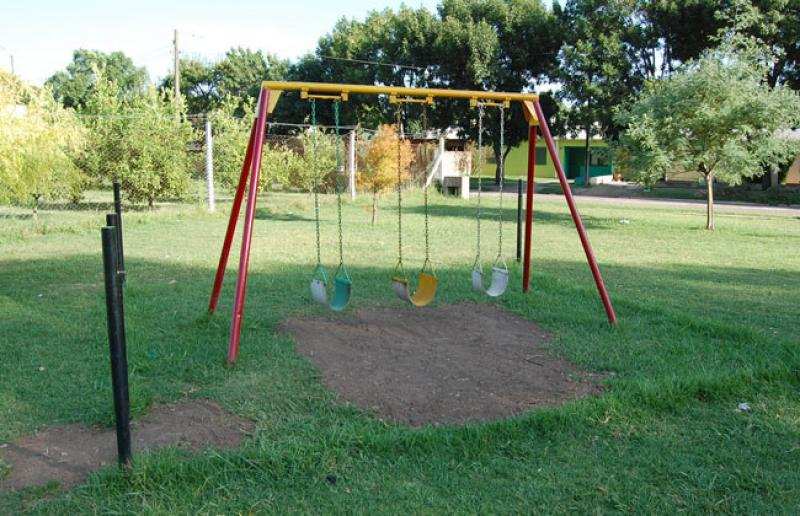
\includegraphics[width=0.4\linewidth]{UT5ej2d}
\end{center}

Considerando que todas las barras están compuestas por el mismo tubular que el emparrillado, se pide:
%
\parte Modelar la estructura con un programa computacional y comparar los resultados con los obtenidos en las partes anteriores en la zona del emparrillado. 


\ejercicio

Sea un emparrillado modificado con respecto al del Ejercicio 2, en el cual se agrega una barra adicional, que está sometida a una carga $q=2$ kN/m, como se muestra en la figura.

\begin{center}
	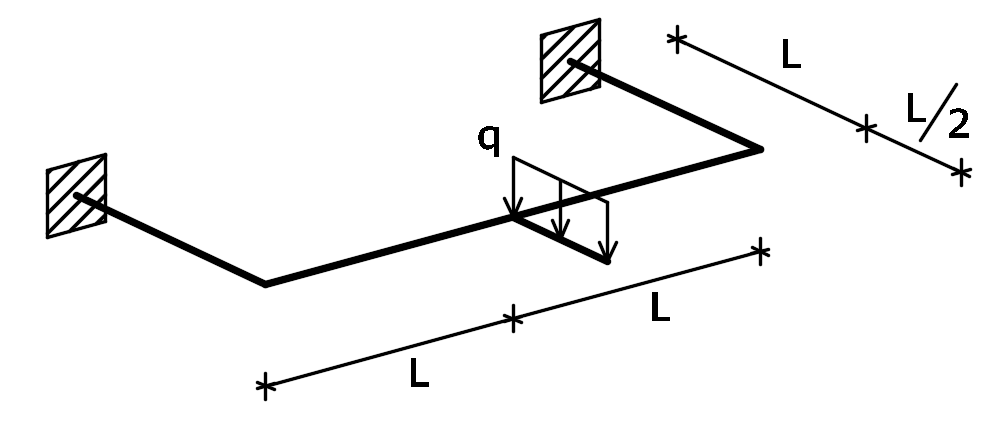
\includegraphics[width=0.6\linewidth]{UT5ej3}
\end{center}

Se pide:
\parte Resolver mediante análisis matricial. Trazar diagramas de solicitaciones.
\parte Comparar resultados obtenidos en a) con los obtenidos utilizando alguna herramienta computacional.


\ejercicio

Sea la estructura mostrada en la figura, construida con barras de acero (E=210 GPa, $\nu=0.3$) de sección circular maciza de diámetro $\phi_{ext}=105$ mm. 

\begin{center}
	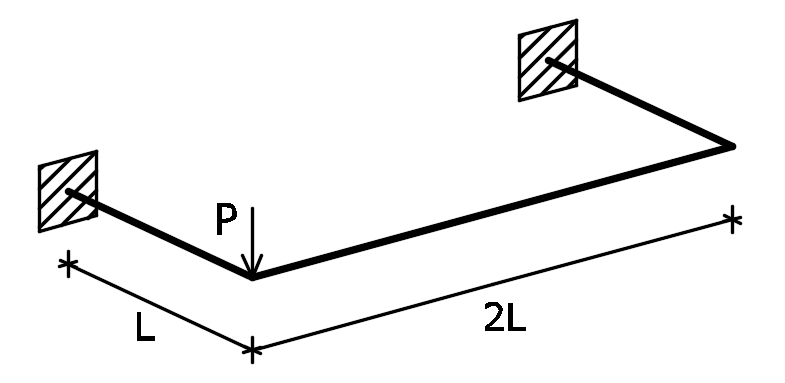
\includegraphics[width=0.6\linewidth]{UT5ej4}
\end{center}

Considerando P=4 kN y L=3.0 m, se pide:

\parte Modificar el código presentado en clase para resolución de emparrillados y obtener desplazamientos y giros nodales. Con los resultados obtenidos trazar diagramas de solicitaciones.
\parte Utilizar algún programa computacional para resolver el problema y verificar los resultados.
\parte Repetir b) descomponiendo en una estructura simétrica y otra antisimétrica.




\ejercicio

La estructura tridimensional de hormigón ($E=30$ GPa y $\nu=0.2$) mostrada en las está conformada por pilares de sección cuadrada $30 \times 30$ cm y vigas de $b=20$ cm y  $h=50$ cm.

\begin{center}
	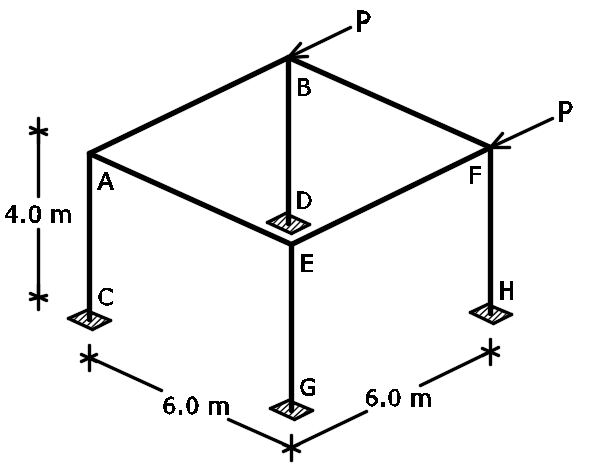
\includegraphics[width=0.45\linewidth]{UT5ej5a}
	\hspace{0.05\linewidth}
	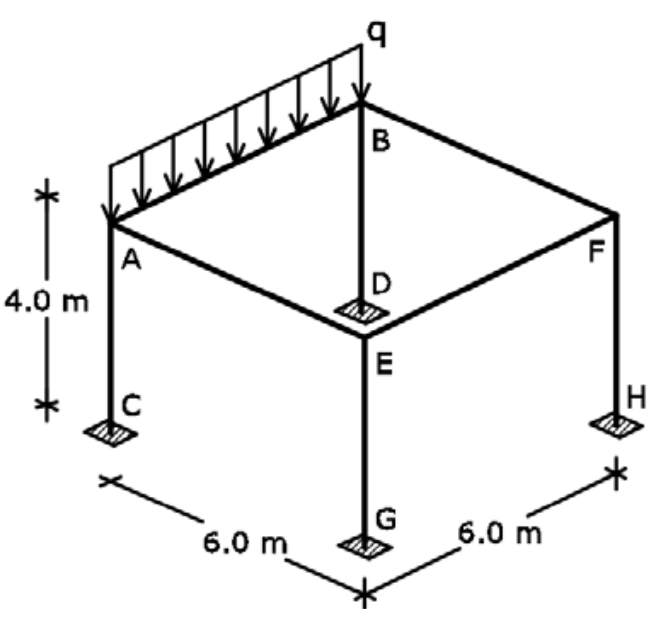
\includegraphics[width=0.45\linewidth]{UT5ej5b}
\end{center}

Para el caso de la estructura a la izquierda se considera $P=20$ kN y se pide:
%
\parte Estudiar los pórticos planos ABCD y EFGH independientes del resto de la estructura en forma analítica. 
%
\parte Modelar la estructura completa en un programa computacional y comparar  los resultados con los hallados en a).

Para el caso de la estructura a la derecha se considera $q=10$ kN/m sobre la viga AB y se pide:
%
\parte Indicar qué modelo plano realizaría para estudiar el pórtico ABCD considerando que los puntos E y F están fijos. Obtener computacionalmente resultados de ese modelo. 
%
\parte Analizar los resultados de modelar la estructura tridimensional y comparar con los obtenidos en c). 

\ejercicio

Se desea estudiar un aerogenerador cuyas dimensiones se muestran en la figura a la izquierda. %
%
%
En la figura a la derecha se muestra un estado de cargas estáticas idealizado de interés para el diseño. Las fuerzas actuantes son:
\begin{itemize}
\item Una fuerza puntual de 80 kN sobre cada punto: F, G y H, representando la fuerza del viento sobre las aspas. 
\item Una fuerza del viento sobre la torre que se ha simplificado como una fuerza en B horizontal de 20 kN. 
\item El peso de las aspas de 30 kN que se aplica como una carga puntual en el punto E.
\item La carga distribuida de 6.5 kN/m que representa el peso de la turbina.
\end{itemize}

Se pide: calcular las reacciones en A y los diagramas de solicitaciones.

\begin{center}
	%	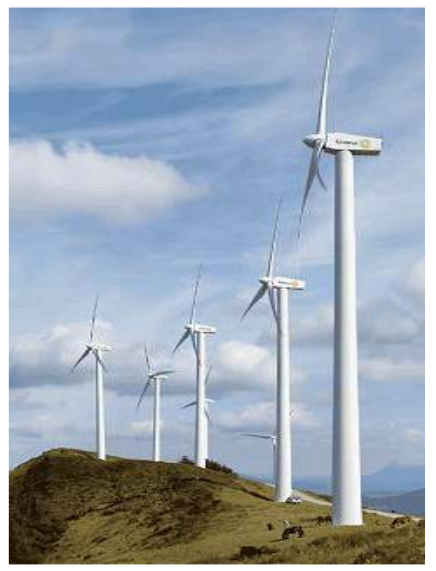
\includegraphics[width=0.2\linewidth]{UT5ej6a}
	%\hspace{0.02\linewidth}
	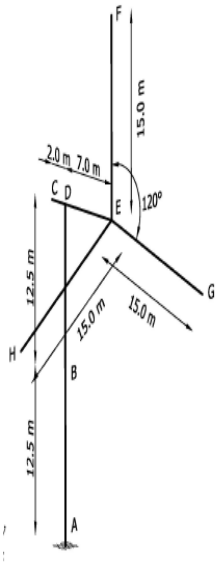
\includegraphics[width=0.35\linewidth]{UT5ej6b}
	\hspace{0.02\linewidth}
	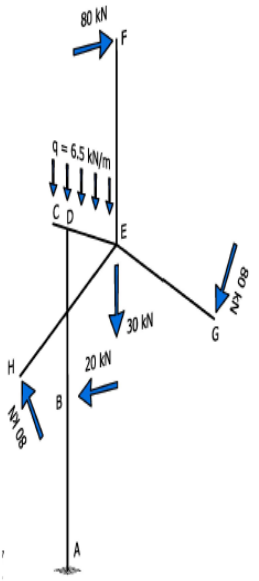
\includegraphics[width=0.35\linewidth]{UT5ej6c}
\end{center}




\ejercicio

Se desea analizar la estructura de un pasamanos considerando un correspondiente Esquema Básico de Cálculo como se muestra en las figuras.

\begin{center}
	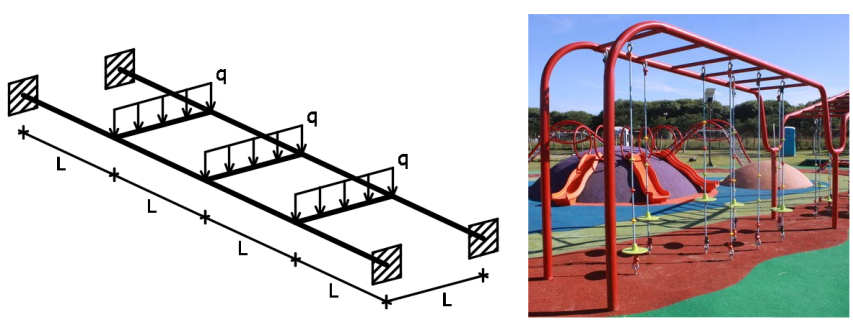
\includegraphics[width=0.85\linewidth]{UT5ej7}
\end{center}

La estructura está compuesta por tubulares de acero ($E=210$ GPa y $\nu=0.3$) de $\phi_{ext}=80$ mm y $t=6$ mm. %
%
Sobre las barras transversales actúa una carga q=3 kN/m y L=1.0 m. Se pide:

\parte Considerar que las barras no presentan rigidez a torsión y calcular analíticamente las solicitaciones en cada una de las barras.
\parte Considerar la rigidez a torsión en las barras y obtener resultados de modelar computacionalmente la estructura.
\parte Comparar resultados obtenidos en a) y b).


\ejercicio (adicional) 

El emparrillado de la figura simula el entrepiso con vigas de una edificación. 

\begin{center}
	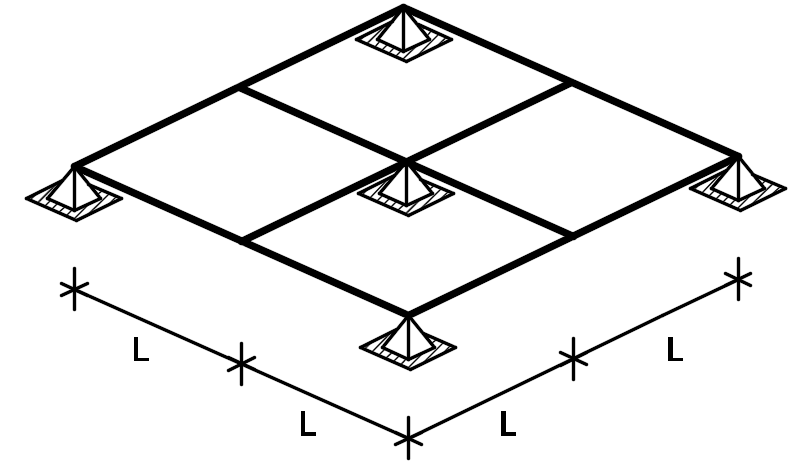
\includegraphics[width=0.65\linewidth]{UT5ej8}
\end{center}

Considerar que todas las vigas son de hormigón (E=30 GPa, $\nu=0.2$) y su sección es 30x80 cm. Las mismas están cargadas con una carga q=15 kN/m y L=5.0 m.

\parte Modelar la estructura computacionalmente. Analizar el comportamiento de las solicitaciones y la deformada.
\parte Si se desprecia la rigidez a torsión de las vigas, ¿cómo se ven afectadas las solicitaciones y deformaciones de las vigas? Analizar.


\ejercicio (adicional) 

La estructura planoespacial mostrada en la figura está formada por barras de misma sección y longitud que el emparrillado del Ejercicio 2.

\begin{center}
	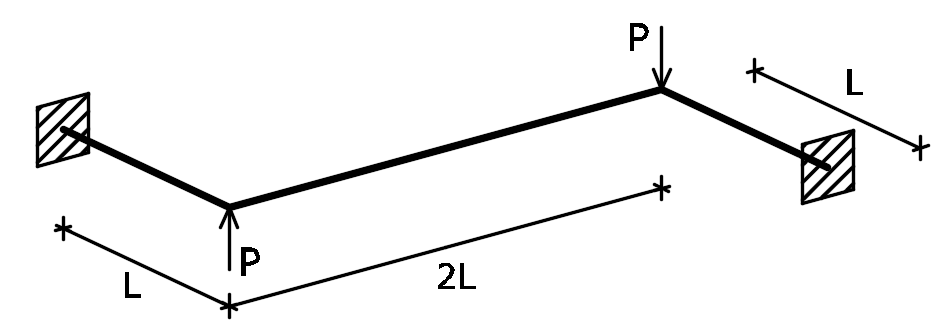
\includegraphics[width=0.75\linewidth]{UT5ej9}
\end{center}

Se pide: trazar diagramas de solicitaciones para $P=10$ kN.

